\documentclass[12pt, french]{article}

\usepackage{fancyhdr, fancybox, lastpage,mhchem}
\usepackage[most]{tcolorbox}
\usepackage[a4paper, margin={0.3in, .75in}]{geometry}
\usepackage{wrapfig}
\pagestyle{fancy}
\renewcommand\headrulewidth{1pt}
\renewcommand\footrulewidth{1pt}
\fancyhf{}
\rhead{ \em{Zakaria Haouzan}}
\lhead[C]{\em{2ème année baccalauréat Sciences Expérimentales}}
\chead[C]{}
\rfoot[C]{}
\lfoot[R]{}
\cfoot[]{\em{Page \thepage / \pageref{LastPage}}}


\newtcolorbox{Box2}[2][]{
                lower separated=false,
                colback=white,
colframe=white!20!black,fonttitle=\bfseries,
colbacktitle=white!30!gray,
coltitle=black,
enhanced,
attach boxed title to top left={yshift=-0.1in,xshift=0.15in},
title=#2,#1}


\begin{document}
\begin{center}
   \shadowbox {\bf{Transformations chimique qui s’effectuent en deux sens
}
 }
\shadowbox{ 	   \bf{Etat d'équilibre d'un système chimique}}

\end{center}

\vspace{-0.2cm}
%%_________________________Exercice ! :"_________________________Exercice
   \begin{Box2}{Exercice 1 :  Acide chlorhydrique}
	On considère un mélange de :

	-Une solution $S_1$ d’acide chlorhydrique de volume $V_1 =5mL$ et de concentration molaire $C_1=0.5mol/L$

	-Une solution $S_2$ d’acide chlorhydrique de volume $V_1 =20mL$ et $pH=1.3$

1. Ecrire l'équation de la réaction chimique d’acide chlorhydrique et l’eau

2. Calculer la quantité de la matière de H3O+ pour chaque solution ? déduire la concentration molaire du
mélange ?

3. Calculer le pH du mélange ?

   \end{Box2}


%%_________________________Exercice !2 :"_________________________Exercice
\begin{Box2}{Exercice 2 :}
%\begin{wrapfigure}{r}{0.22\textwidth}
  %\begin{center}
	  %\vspace{-0.6cm}
	%\includegraphics[width=0.22\textwidth]{./img/Ex2.png}
  %\end{center}
%\end{wrapfigure}

	Le pH de la solution d’acide méthanoïque $HCOOH$ de concentration $C=1,0.10^{-1}moL/L$ est $pH=2.4$

1. Ecrire l'équation de la réaction chimique d’acide méthanoïque avec l’eau ?

2. Dresser le tableau d'avancement de la réaction chimique ?

3. Montrer que la réaction chimique n’est pas totale ?

4. Calculer les concentrations molaires finales des ions de la solution à l’état final de la réaction chimique? (on
néglige les ions $HO^-$)


\end{Box2}

%%_________________________Exercice ! 3:"_________________________Exercice
\begin{Box2}{Exercice 3 : }
%\begin{wrapfigure}{r}{0.5\textwidth}
  %\begin{center}
	%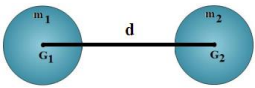
\includegraphics[width=0.5\textwidth]{./img/ex3.png}
  %\end{center}
%\end{wrapfigure}
	Le pH d’une solution aqueuse d’ibuprofène $C_{13}H_{18}O_2$ de concentration molaire $C = 5,0.10^{-2} mol.L^{-1}$ vaut $pH = 2,7$
	à $25^{\circ}C$.

1. Ecrire l'équation de la réaction modélisant la transformation entre l’ibuprofène et l'eau

2. Déterminer l’avancement final $x_f$ en fonction de pH et V

3. Déterminer xm en fonction C et V

4. Montrer que cette transformation est limitée.


\end{Box2}

%%_________________________Exercice 4 : _________________________Exercice
\begin{Box2}{Exercice 4 : }
   % \begin{wrapfigure}[12]{r}{0.5\textwidth}
  %\begin{center}
	  %\vspace{-0.6cm}
	%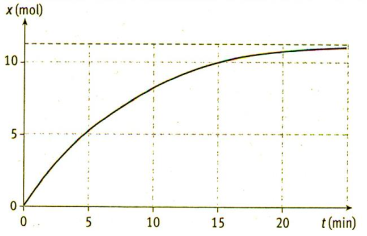
\includegraphics[width=0.5\textwidth]{./img/ex4.png}
  %\end{center}
%\end{wrapfigure}
L'acide propanoïque $C_2H_5COOH$ est un acide gras, utilisé dans la synthèse de certains produits organiques et
pharmaceutiques, de parfums et dans la médecine vétérinaire.

1. On considère, à 25°C, une solution aqueuse (S) d’acide propanoïque de concentration molaire $C =2,0.10^{-3}mol.L^{-1}$ et de volume $V =1,0 L$. La mesure de la conductivité $\sigma$ de la solution (S) a donné la valeur $\sigma = 6,2.10^{-3} S.m^{-1}$.
$$\lambda_{H_3O^+} = 35.10^{-3}S.m^2/mol \hspace{1cm} \lambda_{C_2H_5COO^-}=3,58.10^{-3}S.m^2/mol$$

1.1. Écrire l’équation chimique modélisant la réaction de l’acide propanoïque avec l’eau.

1.2. Dresser le tableau d’avancement de la réaction en utilisant les grandeurs $C_A$, $V_A$, l'avancement $x$ et l'avancement $x_{eq}$ à l'état d’équilibre du système chimique. Déterminer la valeur de l'avancement maximal.

1.3. Vérifier que la valeur de l'avancement à l'état d’équilibre est $1, 6.10^{-4} mol$ .

1.4. Calculer la valeur du taux d'avancement final.

2- On considère une solution aqueuse (S') d'acide propanoïque de concentration molaire $C_A$=$2.10^{-4} mol.L^{-1}$ et de
$pH = 4, 3$ . On note $\tau'$ le taux d'avancement final de la réaction de l'acide propanoïque avec l'eau dans ce cas.

2.1. Déterminer la valeur de $\tau'$ .

2.2. Comparer les valeurs de $\tau$ et $\tau'$ . Déduire.


\end{Box2}
\vspace{-0.8cm}
\begin{center}
   \Large{ \em{Exercices Supplémentaires}}
\end{center}


\vspace{-0.6cm}
%%_________________________Exercice 5 : _________________________Exercice
\begin{Box2}{Exercice 4 : }
   % \begin{wrapfigure}[14]{r}{0.5\textwidth}
  %\begin{center}
	  %\vspace{-0.6cm}
	%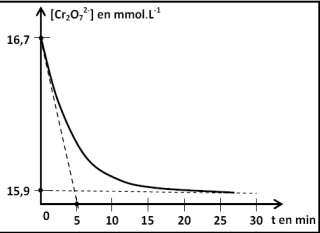
\includegraphics[width=0.5\textwidth]{./img/ex5.png}
  %\end{center}
%\end{wrapfigure}
	On considère une solution $(S_a)$ d’acide méthanoïque de volume V et de concentration molaire $C_a$=$ 10^{-2} mol/L$.
La mesure du pH de cette solution donne : $pH = 2,9$.
On modélise la réaction entre l’acide méthanoïque et l’eau par l’équation suivante :
\vspace{-0.4cm}
$$\ce{HCOOH_{(aq)} + H_2O_{(aq)} <=> HCOO^-_{(aq)} + H_3O^+_{(aq)} }$$

1. Construire le tableau d’avancement de l’évolution du système.

2. Montrer que le taux d’avancement final de cette transformation s’écrit sous la forme $\tau $=$ \frac{10^{-pH}}{C_a}$.Calculer la valeur de $\tau$, et conclure.

\end{Box2}

\begin{Box2}{Exercice 5 : }
On note l’acide Ibuprofène par RCOOH et sa base conjuguée par $RCOO^-$. $M(RCOO^-) = 206g/mol$.

On dissout, dans l'eau pure, un échantillon de masse $m = 200 mg$ d'acide $RCOOH$, contenu dans un sachet
d'Ibuprofène, pour obtenir une solution aqueuse $(S_0)$ de concentration $C_0$ et de volume $V0 $=$ 100 mL$.

1.1. Calculer $C_0$.

1.2. La mesure du pH de la solution $S_0$ a donné la valeur : $pH = 3,17$.

1.2.1 Vérifier, à l'aide du tableau d'avancement, que la réaction de l’Ibuprofène avec l'eau est limitée.

\end{Box2}


\begin{Box2}{Exercice 6 : }

On désignera l’acide étudié par AH et sa base conjuguée par $A^-$ 

On prépare une solution (SA) d’acide butanoïque de concentration molaire $C_A$=$ 10^{-2} mol/L$ et de volume $V_A$.
La mesure du pH de la solution $(S_A)$ donne $pH = 3,41$.

1. Construire le tableau d’avancement.

2. Donner l’expression de l’avancement $x_{eq}$ à l’équilibre en fonction de $V_A$ et $[H_3O^+]_{eq}$ (Concentration molaire
des ions hydroniums à l’équilibre)

3. Trouver l’expression du taux d’avancement final $\tau$ à l’équilibre en fonction de $pH$ et $C_A$, puis calculer sa
valeur. Que conclure ?


\end{Box2}


\begin{Box2}{Exercice 7 : }
	Les conductivités molaires ioniques : $\lambda_{H_3O^+}$=$3,49.10^{-2}S.m^2/mol$ ; $\lambda_{CH_3COO^-}$=$4,09.10^{-3}S.m^2/mol$

	On dispose de deux solutions (S1) et (S2) d’acide éthanoïque.

	La conductivité de la solution (S1) de concentration molaire $C_1=5.10^{-2}mol/L$ ; $\sigma_1= 3,5.10^{-2}S/m$.

	La conductivité de la solution (S2) de concentration molaire $C_2=5.10^{-3}mol/L$ ; $\sigma_2=1,1.10^{-2}S/m$.

	On considère que la dissolution de l’acide éthanoïque dans l’eau est limitée.

1. Ecrire l’équation modélisant la dissolution de l’acide éthanoïque dans l’eau.

2. Trouver l’expression de la concentration molaire effective $[H_3O^+]_{(eq)}$ des ions oxoniums à l’équilibre en
fonction de $\sigma$ et $\lambda_{CH_3COO^-}$ et $\lambda_{H_3O^+}$.

3. Calculer $[H_3O^+]_{(eq)}$ dans chacune des solutions (S1) et (S2).

4. Déterminer les taux d’avancement final $\tau_1$ et $\tau_2$ de la réaction de l’acide éthanoïque avec l’eau dans chacune
des solutions (S1) et (S2). Déduire l’influence de la concentration initiale de la solution sur le taux
d’avancement final.

\end{Box2}
\end{document}
